%%%%%%%%%%%%%%%%%%%%%%%%%%%%%%%%%%%%%%%%%%%%%%%%%%%%%%%%%%%
% --------------------------------------------------------
% Tau
% LaTeX Template
% Version 2.4.1 (22/05/2024)
%
% Author: 
% Guillermo Jimenez (memo.notess1@gmail.com)
% 
% License:
% Creative Commons CC BY 4.0
% --------------------------------------------------------
%%%%%%%%%%%%%%%%%%%%%%%%%%%%%%%%%%%%%%%%%%%%%%%%%%%%%%%%%%%
\documentclass[9pt,a4paper,twoside]{tau-class/tau}

%----------------------------------------------------------
% TITLE
%----------------------------------------------------------

\usepackage{enumitem}
\newcount\NewCount

\journalname{ESCOM}
\title{Cellular Automata}


%----------------------------------------------------------
% AUTHORS, AFFILIATIONS AND PROFESSOR
%----------------------------------------------------------

\author[a]{Diego Castillo Reyes}
\author[a]{Marthon Leobardo Yañez Martinez}
\author[a]{Aldo Escamilla Resendiz}
\author[a]{Muñoz González Eduardo}

%----------------------------------------------------------

\affil[a]{Researcher}


\professor{Dra. Miriam Pescador Rojas}

%----------------------------------------------------------
% FOOTER INFORMATION
%----------------------------------------------------------

\institution{Escuela Superior de Cómputo, IPN}
\footinfo{Cellular Automata}
\theday{June 21, 2024}
\course{Genetic Algorithms}

%----------------------------------------------------------
% ABSTRACT AND KEYWORDS
%----------------------------------------------------------

\begin{abstract}    
    Cellular automata are a mathematical and computational model used to simulate dynamic systems. 
        This work presents a review of cellular automata, their history, classification, and applications. 
        Additionally, an example of one-dimensional and two-dimensional cellular automata is shown.
\end{abstract}

%----------------------------------------------------------

\keywords{Automata, Cellular, Genetic, Algorithms, Simulation}

%----------------------------------------------------------

\begin{document}	
    \maketitle 
    \thispagestyle{firststyle} \tauabstract
    \tableofcontents
%----------------------------------------------------------

\section{Introduction}

    Cellular automata (CA) are \textit{discrete, abstract computational systems} that have proved useful both as general models of complexity and as more specific representations of non-linear dynamics in a variety of scientific fields. 

    Firstly, CA are typically spatially and temporally discrete. They are composed of a finite or denumerable set of homogeneous, simple units called cells. At each time unit, the cells instantiate one of a finite set of states. 
    They evolve in parallel at discrete time steps, following state update functions or dynamical transition rules. 
    The update of a cell's state is obtained by taking into account the states of cells in its local neighborhood, meaning there are no actions at a distance.

    Secondly, CA are abstract. They can be specified in purely mathematical terms, and physical structures can implement them.

    Thirdly, CA are computational systems. They can compute functions and solve algorithmic problems. Despite functioning differently from traditional 
    Turing machine-like devices, CA with suitable rules can emulate a universal Turing machine\footnote{\cite[The Stanford Encyclopedia of Philosophy (Winter 2021 Edition), Edward N. Zalta (ed.)]{sep-touring-machine}}, 
    and therefore compute anything that is computable according to Turing's thesis.\cite{sep-cellular-automata}


\section{Background}


    The concept of cellular automata was invented by Stansilaw Ulam and John Von Neumann in
    the 1940s while they were working at the Los Alamos National Laboratory.
    The work on cellular automata began in the 1940s, with significant developments occuring throughout
    that decade. Von Neumann’s comprehensive work on self-replicating automata was published 
    posthumously in 1966 in the book ``Theory of Self-Reproducing Automata'', edited by 
    Arthur W. Burks.

    A cellular automaton (CA) is a one-dimensional array (which can be infinitely long in both directions) of cells. 
    Time progresses in discrete steps, and at each step, every cell is in one of a finite number of possible states. The state of each cell changes at each tick of the clock, and this new state is determined entirely by the current state of the cell and its immediate left and right neighbors. 
    This state change is governed by a function called the local rule, which is identical for all cells. 
    The CA operates autonomously without any external input. 
    The collection of all cell states at any given time is referred to as the configuration or global state of the CA, 
    representing its stage of evolution. Starting from an initial configuration at time t = 0, the CA evolves deterministically according to the local 
    rule applied to each cell at each clock tick. (see Fig. \ref{fig:timeStep})

    When the local rule is applied to each cell, it transforms the entire set of configurations into itself. 
    This transformation is known as the global map or global rule of the CA. This description captures the essence of a CA, which is a widely studied structure.
    \begin{figure}[H]
        \centering
        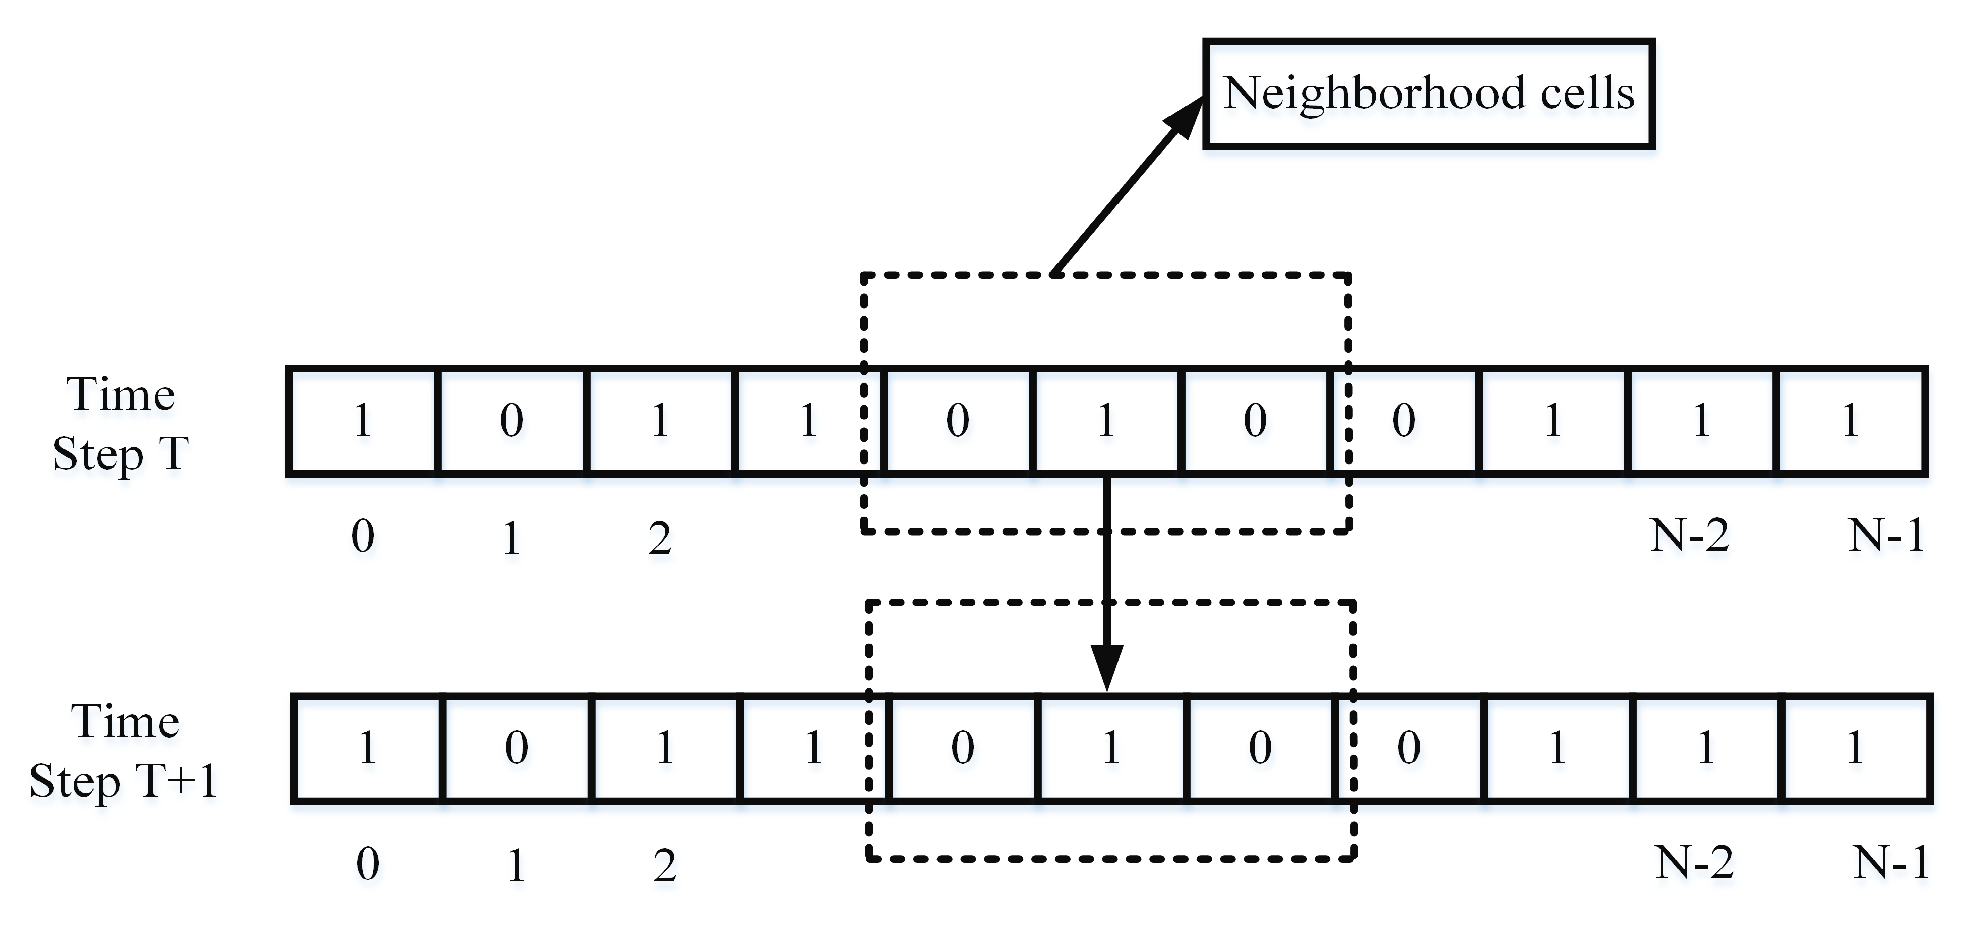
\includegraphics[width=0.75\columnwidth]{figures/timestep.png}
        \caption{Evolution of a CA at each time step. \cite{math11102322}}
        \label{fig:timeStep}
    \end{figure}

    The automaton initially described by von Neumann\cite{von-neumann-automata} consists of a two-dimensional infinite array of uniform cells, with each cell connected to its four orthogonal neighbors. 
    This structure was originally termed a cellular space, though the term CA is now more commonly used. Von Neumann introduced this concept as a formal model for self-reproducing biological systems. His key ideas can be traced back to his earlier work on modeling biological systems. 
    Von Neumann aimed to apply the rigor of axiomatic and deductive methods to the study of complex natural systems. His concept of a self-reproducing automaton is a remarkable adaptation of the idea behind constructing a universal Turing Machine (TM).

    \begin{figure}[H]
        \centering
        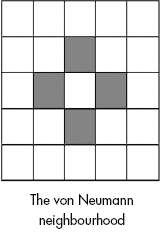
\includegraphics[width=0.75\columnwidth]{figures/vonNeumann.png}
        \caption{Von Neumann's cellular automaton.}
        \label{fig:vonNeumann}
    \end{figure}


    \subsection{One-Dimensional Cellular Automata}


    Most of the dynamic features of cellular automata can be observed in the study of the one-dimensional case. In this context, we define the neighborhood of a cell \( c \) with a radius \( r \) as the \( r \) cells to the left of \( c \) and the same number of cells to the right of \( c \). Including \( c \) itself, this neighborhood comprises \( 2r + 1 \) cells. For the simplest case where \( r = 1 \) and \( k = 2 \) (the allowable states), a three-cell neighborhood with two possible states (0 and 1) for each cell can be expressed in \( 2^3 = 8 \) different ways. All eight neighborhood states with \( r = 1 \) and \( k = 2 \) are illustrated in Figure \ref{fig:neighborhood_states}, and in general, there are \( k^{2r+1} \) one-dimensional neighborhood states.\cite{schiff2007}
    
        \begin{figure}[H]
            \centering
            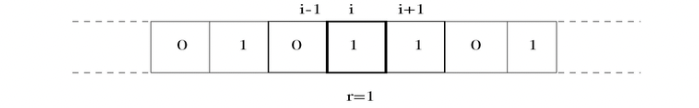
\includegraphics[width=0.9\columnwidth]{figures/transition_rule.png}
            \caption{Eight possible neighborhood states with \( r = 1 \) and \( k = 2 \).}
            \label{fig:neighborhood_states}
        \end{figure}
    Let us adopt the notation \( c_i(t) \) to denote the state of the \( i \)-th cell at time \( t \) (Figure \ref{fig:cell_states}).
    
    
    \begin{figure}[H]
        \centering
        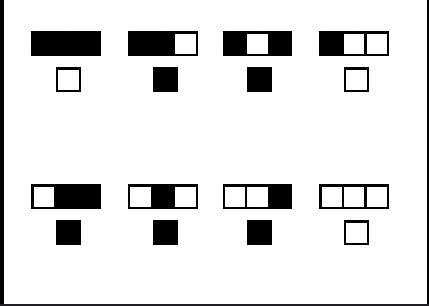
\includegraphics[width=0.45\columnwidth]{figures/rule_graphic.png}
         \caption{State of the \( i \)-th cell at time \( t \).} 
        \label{fig:cell_states}
    \end{figure}


    At the next time step, \( t + 1 \), the cell state will be \( c_i(t + 1) \). Mathematically, we can express the dependence of a cell’s state at time step \( t + 1 \) on the states of its left and right nearest neighbors \( c_{i-1}(t) \) and \( c_{i+1}(t) \) at time step \( t \) by the relation

    \begin{equation}
        c_i(t + 1) = \phi \left( c_{i-1}(t), c_i(t), c_{i+1}(t) \right),
    \end{equation}

    where \( \phi \) is the local transition function. For example, consider the simple transition rule

    \begin{equation}
        c_i(t + 1) = \left( c_{i-1}(t) + c_i(t) + c_{i+1}(t) \right) \mod 2,
        \label{eq:transition_rule}
    \end{equation}

    where $\mod 2$ means taking the remainder after dividing the indicated sum by 2, resulting in either 0 or 1. We can put this rule into a transition table format by computing \( c_{i-1}(t) + c_i(t) + c_{i+1}(t) \mod 2 \) for the eight possible input values:

    \begin{table}[H]
        \centering
        \begin{tabular}{cccc}
            \toprule
            $c_{i-1}(t)$ & $c_i(t)$ & $c_{i+1}(t)$ & $c_i(t + 1)$ \\
            \midrule
            1 & 1 & 1 & 1 \\
            1 & 1 & 0 & 0 \\
            1 & 0 & 1 & 0 \\
            1 & 0 & 0 & 1 \\
            0 & 1 & 1 & 0 \\
            0 & 1 & 0 & 1 \\
            0 & 0 & 1 & 1 \\
            0 & 0 & 0 & 0 \\
            \bottomrule
        \end{tabular}
        \caption{Transition table for the rule \( c_i(t + 1) = (c_{i-1}(t) + c_i(t) + c_{i+1}(t)) \mod 2 \).}
        \label{tab:transition_table}
    \end{table}

    A very convenient way to illustrate the allowable rules for one-dimensional cellular automata with \( r = 1 \) and \( k = 2 \) is to indicate the state (color) of the middle cell at the next time step, given the state (color) of itself and its two nearest neighbors (Figure \ref{fig:cell_states}).

    Here, the middle cell at time \( t \) (in the top row) has its state altered according to the states of its two nearest neighbors and its own state to yield the cell’s new state at time \( t + 1 \) (bottom row). This also represents the rule in Equation \ref{eq:transition_rule}. Observe that in four of the eight cases, a black cell appears. One consequence of this is that if we took a disordered array of a large number of cell sites, then the average fraction (or density) of black cell sites that evolve after one iteration will be 0.5.

    The cellular automaton defined by this rule has the graphical representation depicted in Figure \ref{fig:rule_graphic}, starting with a single black cell with each subsequent generation of the automaton appearing on the next line down.
    \begin{figure}[H]
        \centering
        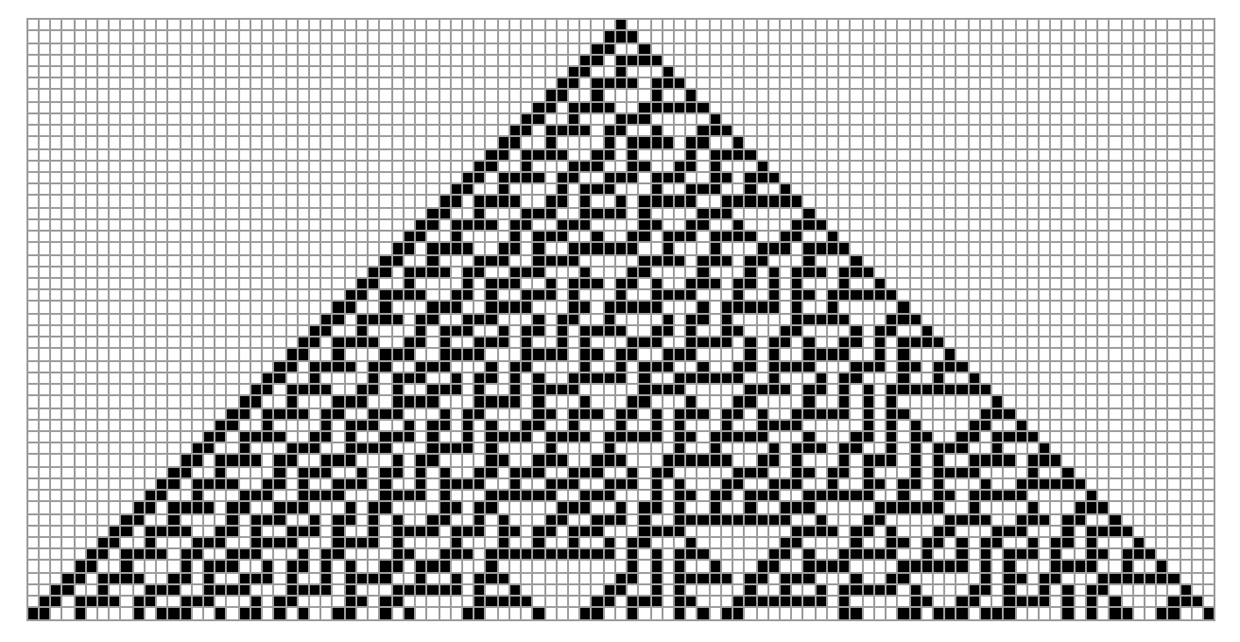
\includegraphics[width=0.75\columnwidth]{figures/rule30.png}
         \caption{Graphical representation of the evolution of the rule starting with a single black cell. Each new line downward represents the evolution of the automaton at the next time step.} 
        \label{fig:rule_graphic}
    \end{figure}

    So, how many possible rules are there for \( r = 1 \) and \( k = 2 \)? Since there are eight possible neighborhood states of three cells and each of these results in two possible state outcomes for the middle cell, there are \( 2^8 = 256 \) possible transition rules by which this can be achieved as seen in Figure~\ref{fig:floatrules}. Wolfram described these as elementary cellular automata.

    \begin{figure*}[tp] % t for position at the top of the current page; b for position at the bottom; p for new page
		\centering
		  \begin{subfigure}[b]{0.38\linewidth} % Fig (a)
			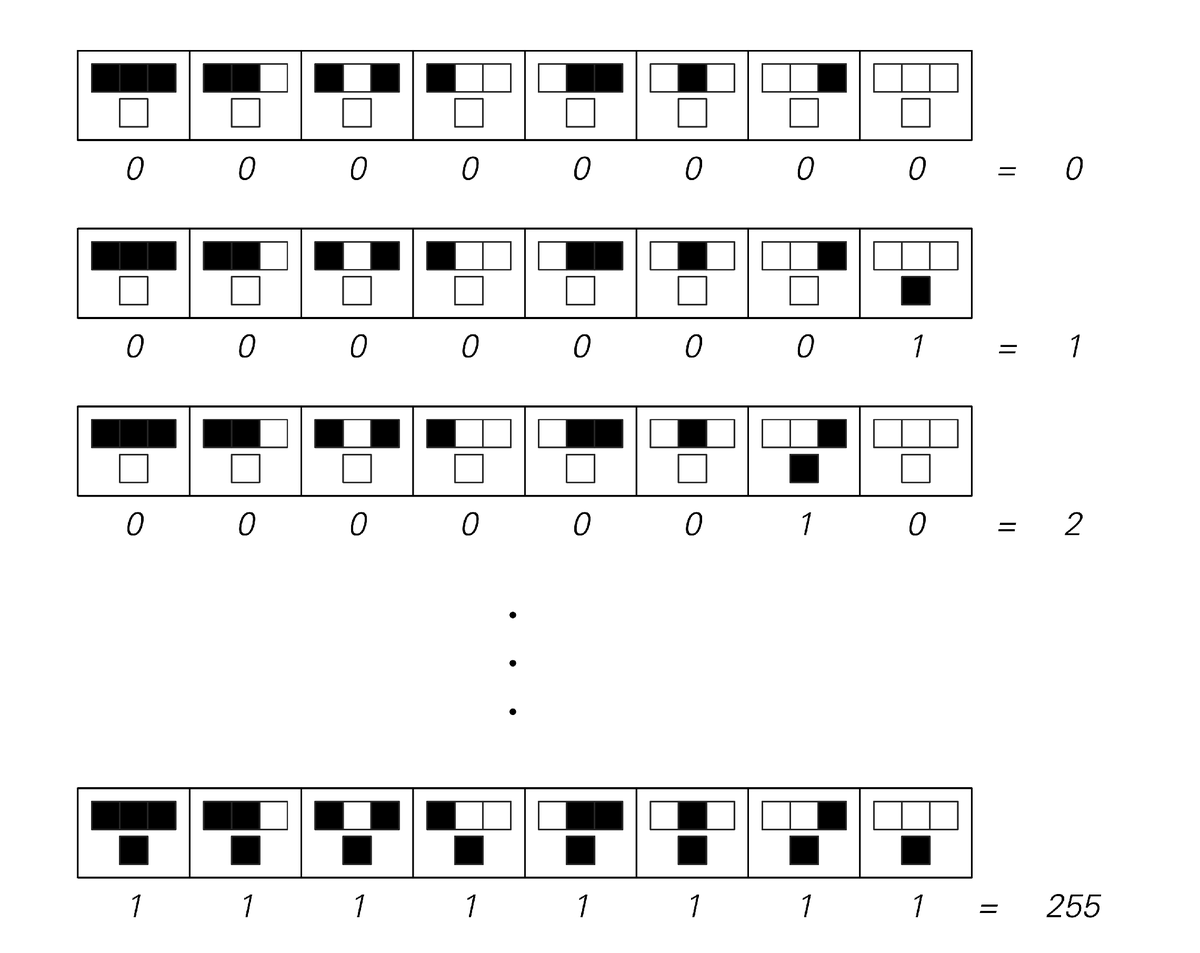
\includegraphics[width=\linewidth]{figures/rules256.png}
			\caption{The 256 rules}
		\end{subfigure}
			\hspace{20pt}   % Space between the figures
		\begin{subfigure}[b]{0.375\linewidth} % Fig (b)
			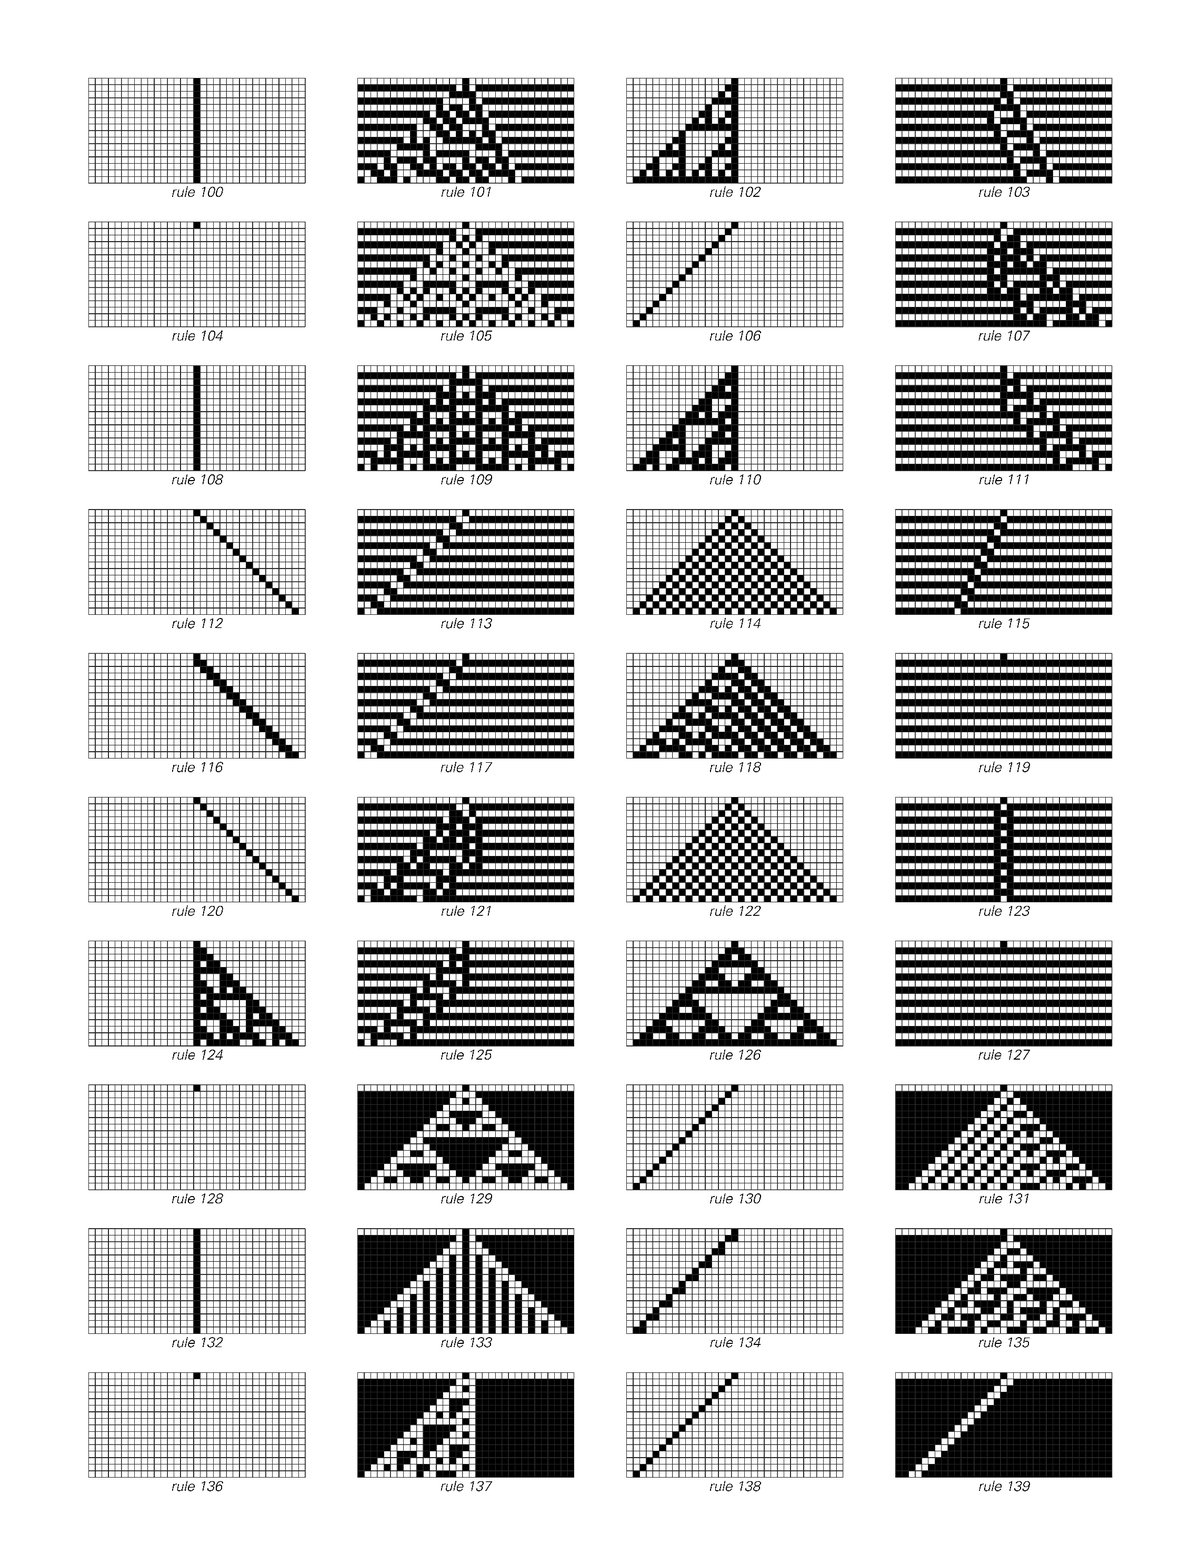
\includegraphics[width=\linewidth]{figures/generetions.png}
			\caption{Genereations for some rules}
		\end{subfigure}
		\caption{The 256 rules and the generations for some of them.}
		\label{fig:floatrules}
	\end{figure*}

    \subsection{Motivation}
    
    
    Cellular automata, a concept derived from computer science, are increasingly employed as models in ecological research. This concept spans a variety of topics, including automata theory and artificial intelligence. 
    Cellular automata, as representations of this concept, create miniature worlds where each cell houses an automaton. The behavior of a cellular automaton can be remarkably complex, often resembling lifelike processes. 
    This complexity has inspired a new field of study known as artificial life or, more cautiously, complex systems. Conferences in this field attract computer and mathematical scientists, as well as a growing number of participants from geography, ecology, geology, and other disciplines, along with a popular audience. 
    Currently, the field of ecology has accumulated sufficient experience with cellular automaton models to move beyond initial simple models and harness the full potential of this tool for comprehensive simulation. 
    However, validation and interpretation continue to be significant challenges in utilizing these models effectively.\cite{DEWDNEY2008541}

    The primary motivation behind cellular automata was to understand and model complex
    systems using simple, local rules. This idea was rooted in the study of biological 
    processes and the desire to create self-replicating machines.

    \subsection{Developments}
  
    John Conway's work (1970s): Conway popularized cellular
    automata with his "Game of Life", a bidimensional binary cellular automaton. 
    This game demonstrated how simple rules could lead to complex emergent behavior, 
    sparking widespread interest and research in cellular automata.

    Stephen Wolfram's work (1980s): Wolfram conducted extensive research on cellular
    automata, classifying them into four types based on their behavior and demonstrating 
    their potential as models of natural processes and as computational systems.
  

    Fig. \ref{fig:figure} An example of Conway's Game of Life.
	\begin{figure}[H]
		\centering
		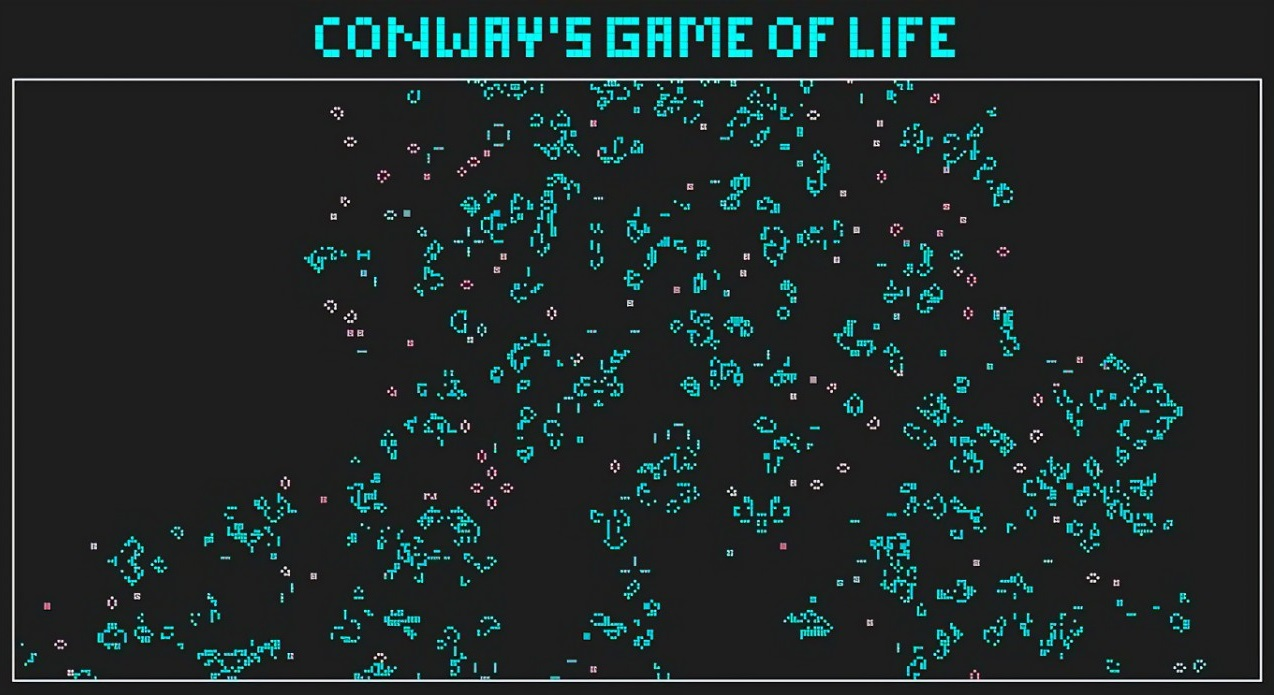
\includegraphics[width=0.75\columnwidth]{figures/gameOfLife.jpg}
		\caption{Conway's Game of Life.}
		\label{fig:figure}
	\end{figure}

    \subsection{Applications}
	
        Cellular automata have been used in various fields, including:
        
        \begin{itemize}
            \item Computer Science: Parallel computation, cryptography, and image processing.
            \item Physics: Modeling physical systems, such as fluid dynamics and crystal growth.
            \item Biology: Simulating biological processes, such as population dynamics and pattern formation.
        \end{itemize}
		
        Fig. \ref{fig:ExampleAutonoma} Application of cellular automata on Computer Science.
	\begin{figure}[H]
		\centering
		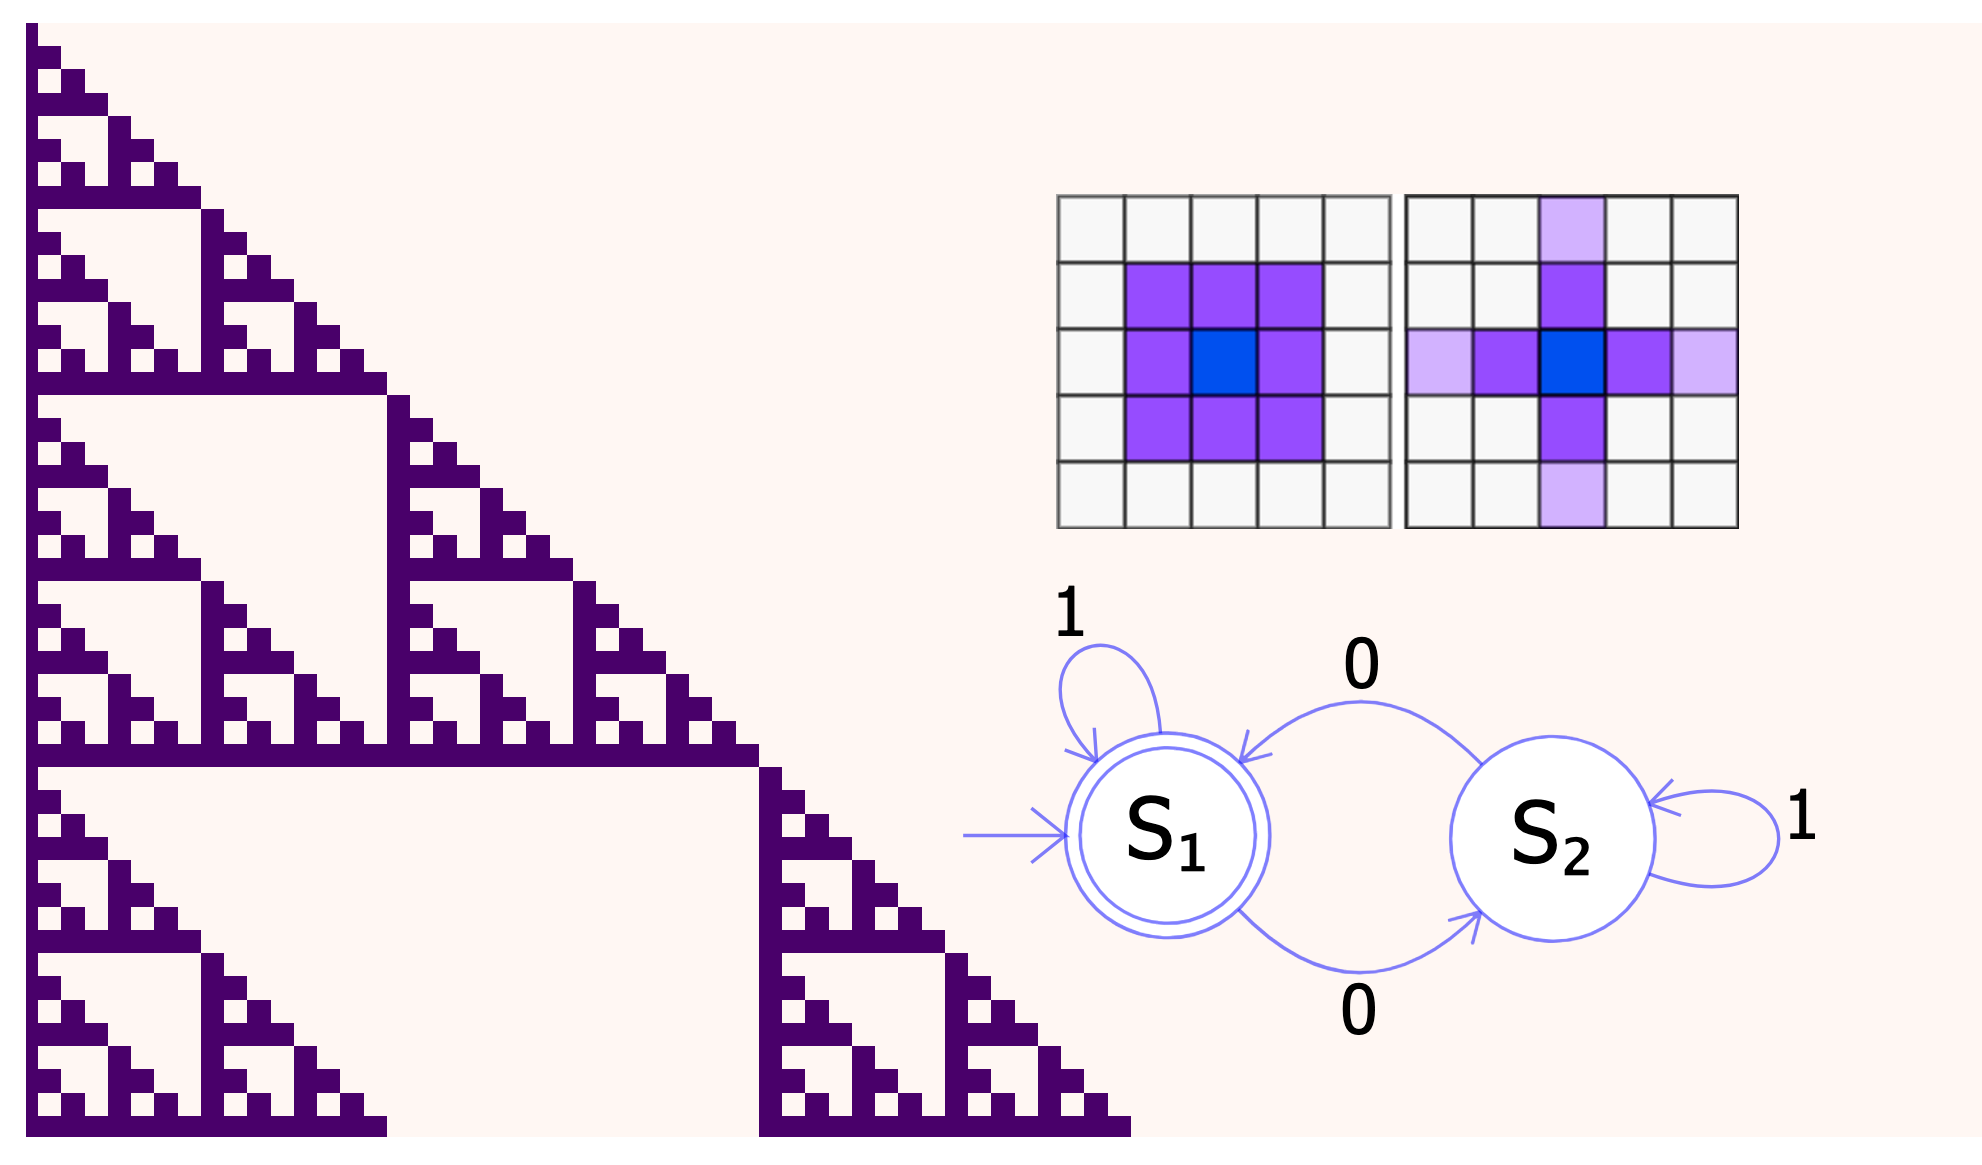
\includegraphics[width=0.75\columnwidth]{figures/theoryOfComputation.png}
		\caption{Example of cellular automata.}
		\label{fig:ExampleAutonoma}
	\end{figure}

\section{Cellular Automata Algorithm}
    \begin{algorithm}
        \caption{Basic Cellular Automaton}
        \KwIn{\texttt{gridWidth}: Width of the grid, \texttt{gridHeight}: Height of the grid, \texttt{states}: Set of possibles states for the cells, \texttt{neighborhood}: Set of relative positions defining the neighborhood of each cell, \texttt{rules}: Set of state transition rules, \texttt{maxTimeSteps}: Maximum number of time steps}
        \KwOut{The final state of the grid}
        
        Initialize \texttt{gridHeight} $\times$ \texttt{gridWidth}, set the initial states on the grid and create \texttt{newGrid} as a copy of the grid.\;
        
        \While{$i$ < \texttt{maxTimeSteps}}{
            \For{$x$ in \texttt{gridWidth}}{
                \For{$y$ in \texttt{gridHeight}}{
                    \texttt{neighbors} = getNeighbors(\texttt{grid}, \texttt{neighborhood}, $x$, $y$)\;
                    \texttt{newGrid}[$x$][$y$] = applyRules(\texttt{grid}[$x$][$y$], \texttt{neighbors}, \texttt{rules})\;
                }
            }
            Display the state of \texttt{newGrid}
            \texttt{grid} = \texttt{newGrid}\;
            $i$++\;
        }
    \end{algorithm}



%%%%%%%%%%%%%%%%%%%%%%%%%%%%%%%%%%%%%%%%%%%%%%%%%%%%%%%%%%%
%%%%%%%%%%%%%%%%%%%%%%%%%%%%%%%%%%%%%%%%%%%%%%%%%%%%%%%%%%%
%%%%%%%%%%%%%%%%%%%%%%%%%%%%%%%%%%%%%%%%%%%%%%%%%%%%%%%%%%%
%%%%%%%%%%%%%%%%%%%%%%%%%%%%%%%%%%%%%%%%%%%%%%%%%%%%%%%%%%%

\section{Parameters Required on a Cellular Automata}



%%%%%%%%%%%%%%%%%%%%%%%%%%%%%%%%%%%%%%%%%%%%%%%%%%%%%%%%%%%
%%%%%%%%%%%%%%%%%%%%%%%%%%%%%%%%%%%%%%%%%%%%%%%%%%%%%%%%%%%
%%%%%%%%%%%%%%%%%%%%%%%%%%%%%%%%%%%%%%%%%%%%%%%%%%%%%%%%%%%
%%%%%%%%%%%%%%%%%%%%%%%%%%%%%%%%%%%%%%%%%%%%%%%%%%%%%%%%%
\section{Versions of Cellular Automata}


%%%%%%%%%%%%%%%%%%%%%%%%%%%%%%%%%%%%%%%%%%%%%%%%%%%%%%%%%%%
%%%%%%%%%%%%%%%%%%%%%%%%%%%%%%%%%%%%%%%%%%%%%%%%%%%%%%%%%%%
%%%%%%%%%%%%%%%%%%%%%%%%%%%%%%%%%%%%%%%%%%%%%%%%%%%%%%%%%%%
%%%%%%%%%%%%%%%%%%%%%%%%%%%%%%%%%%%%%%%%%%%%%%%%%%%%%%%%%
\section{Analogy with the Nature}
    

%%%%%%%%%%%%%%%%%%%%%%%%%%%%%%%%%%%%%%%%%%%%%%%%%%%%%%%%%%%
%%%%%%%%%%%%%%%%%%%%%%%%%%%%%%%%%%%%%%%%%%%%%%%%%%%%%%%%%%%
%%%%%%%%%%%%%%%%%%%%%%%%%%%%%%%%%%%%%%%%%%%%%%%%%%%%%%%%%%%
%%%%%%%%%%%%%%%%%%%%%%%%%%%%%%%%%%%%%%%%%%%%%%%%%%%%%%%%%
\section{Implementation Repositories}



%%%%%%%%%%%%%%%%%%%%%%%%%%%%%%%%%%%%%%%%%%%%%%%%%%%%%%%%%%%
%%%%%%%%%%%%%%%%%%%%%%%%%%%%%%%%%%%%%%%%%%%%%%%%%%%%%%%%%%%
%%%%%%%%%%%%%%%%%%%%%%%%%%%%%%%%%%%%%%%%%%%%%%%%%%%%%%%%%%%
%%%%%%%%%%%%%%%%%%%%%%%%%%%%%%%%%%%%%%%%%%%%%%%%%%%%%%%%%
\section{Usage Examples}
In the following section, we present some articles where you can find implementations of cellular automata.

\subsection{ A computational tumor growth model experience based on molecular dynamics point of view using deep cellular automata }

The article \textit{A computational tumor growth model experience based on molecular dynamics point of view using deep cellular automata} discusses a novel approach to modeling cancerous tumor growth by integrating cellular automata (CA) with deep learning techniques, particularly convolutional neural networks (CNNs). This integration aims to leverage the strengths of both methods to create a robust and scalable solution for simulating tumor development.\cite{MATIN2024102752}

\subsubsection{Overview of Cellular Automata and CNN Integration}

Cellular automata are dynamic systems composed of a grid of cells, each of which can be in one of several states. The state of each cell at any given time is determined by a set of rules that consider the states of neighboring cells. Traditional CA models operate based on predetermined rules, which can be rigid and may not adapt well to varying conditions. By contrast, when CA rules are implemented within a CNN framework, these rules can potentially be learned from data, making the system adaptive and capable of handling more complex and varied scenarios.

\subsubsection{Implementation Details}

The article details how the CA is represented as a CNN. The process involves defining the CA as a mapping between possible pixel configurations in a binary image and corresponding output pixel values. This mapping is applied to randomly generated binary images to create training data, which are then used to train the CNN. The network architecture typically involves a 3 $×$ 3 convolution layer followed by several 1 $×$ 1 convolution layers. This setup allows the network to perform local operations repeatedly, mimicking the behavior of CA.

The integration of CA with CNNs provides several advantages:

\begin{itemize}
    \item \textbf{Scalability}: Leveraging the parallel processing capabilities of modern GPUs optimized for CNN operations allows for faster simulations and predictions, especially for large grid sizes.
    \item \textbf{Granular Predictions}: By integrating CA rules within a CNN framework, it is possible to achieve detailed predictions at the cellular level. This granularity is crucial for applications like tumor growth prediction, where understanding cellular interactions at a micro-level can provide invaluable insights.
    \item \textbf{Adaptability}: Unlike traditional CA models that are constrained by predefined rules, the CNN-based approach allows for the rules to be learned from data, enhancing the system's ability to generalize and adapt to different conditions.
\end{itemize}

\subsubsection{Results and Validation}

The proposed model was validated by comparing its output to established mathematical models of tumor growth, specifically the Gompertz growth model. The results showed that the CNN-CA model aligns well with the Gompertz model, demonstrating its accuracy and robustness. Additionally, the model was tested on various tumor growth datasets, highlighting its versatility and predictive capabilities.

This research paves the way for more sophisticated and adaptable models in the field of tumor growth simulation, offering a promising direction for future studies in oncology.

\subsection{Implementing Fuzzy Cellular Automata in Breast Cancer Image Segmentation}

The article \textit{Breast Cancer Images Segmentation using Fuzzy Cellular Automaton} presents an innovative approach for segmenting breast cancer images by integrating Cellular Automata (CA) with Fuzzy Logic, resulting in the so-called Fuzzy Cellular Automaton. This method aims to enhance the accuracy and flexibility of segmenting the mass region in mammograms, achieving highly promising results with an accuracy of 98.66\% on the mini-MIAS dataset.\cite{ION2023999}

\subsubsection{Overview of Cellular Automata and Fuzzy Logic Integration}

Cellular Automata (CA) are dynamic systems comprised of a grid of cells, each of which can be in one of several states. The state of each cell at any given time is determined by a set of rules that consider the states of neighboring cells. Traditional CA models operate based on predetermined rules, which can be rigid and may not adapt well to varying conditions. By incorporating Fuzzy Logic into CA, the model gains the ability to categorize pixels more flexibly, enhancing its adaptability to different imaging scenarios.

\subsubsection{Implementation Details}

The article outlines how CA is combined with Fuzzy Logic to form a Fuzzy Cellular Automaton. This process involves several key steps:

\begin{enumerate}
    \item \textbf{Preprocessing}: The mammogram images are converted to grayscale, and noise is reduced using Gaussian Blur and Binary Threshold techniques. Background and pectoral muscle removal are performed to isolate the region of interest (ROI).

    \item \textbf{Segmentation}: An improved version of the CA algorithm is applied to the preprocessed images. The segmentation starts with a pixel (seed) and expands to neighboring pixels with similar shades, computing the strength of the neighboring cells based on the CA rules. 

    \item \textbf{Fuzzy Logic Integration}: To refine the segmentation, Fuzzy Logic is applied. Two fuzzy sets are constructed based on the grayscale distributions of the strength determined by the CA algorithm. These sets model the presence of a certain pixel in the suspicious region and the contrary event.
\end{enumerate}

\subsubsection{Advantages of the Approach}

Integrating CA with Fuzzy Logic offers several advantages:

\begin{itemize}
    \item \textbf{Improved Accuracy}: The method achieves a high accuracy rate of 98.66\% on the mini-MIAS dataset, significantly improving the precision of mass region segmentation.
    \item \textbf{Flexibility}: Fuzzy Logic provides a more adaptable technique for pixel categorization, allowing the model to handle variations in imaging conditions more effectively.
    \item \textbf{Visual Clarity}: The visually progressive nature of CA, combined with the adaptability of Fuzzy Logic, results in clearer and more interpretable segmentation results for medical specialists.
\end{itemize}

\subsubsection{Experimental Results}

The proposed approach was validated on the mini-MIAS dataset, comprising 322 mammograms, 118 of which contain suspicious masses. The results showed that the Fuzzy Cellular Automaton outperformed the traditional CA approach, with a mean Intersection over Union (IoU) score of 83.79\%, compared to 65.11\% for the CA approach.


\addcontentsline{toc}{section}{References}
\printbibliography

\end{document}